\thispagestyle{empty}
\chapter{Bioinformatics and Genetics provide a robust framework for investigating genomes evolution}
{\hypersetup{linkcolor=GREYDARK}\minitoc}
\label{chap:intro-biol_evol}

Since Jean Baptiste Lamarck in 1809~\citep{lamarck_philosophie_1809} molecular evolutionary biology became a scientific discipline regrouping researchers and expanding its results beyond empirical observations and theoretical postulations to encompass protocols, experiments, and mathematical models with genetic as the raw material (see `\nameref{chap:intro-evol_forces}' chapter). This discipline is dedicated to study the genetic variations among species and within populations with the idea that all species have a shared ancestor. Central to evolutionary biology is the study of evolutionary forces that shape the characteristics of species and populations. Through rigorous examination of these factors, evolutionary biology seeks to gain profound insights into the dynamic processes driving the evolution of life on Earth.

Notably, evolutionary biology has made substantial contributions to diverse domains such as unraveling our historical origins~\citep{cann_mitochondrial_1987, vigilant_african_1991, krause_derived_2007, somel_microrna-driven_2011, callaway_oldest_2021}, our cultural development~\citep{pagel_wired_2013}, and even the evolution of languages~\citep{nettle_genetic_2003, levinson_tools_2012}. Furthermore, the influence of evolutionary biology has now expanded to encompass areas such as pharmaceutical research and biomedical applications, including cancer research~\citep{casas-selves_how_2011, crespi_evolutionary_2005}. 
\textit{`Nothing in Biology Makes Sense Except in the Light of Evolution' by Theodosius Dobzhansky (1973)}, remains profoundly resonant and highlights the pervasive role of evolution in elucidating biological phenomena across various disciplines.

Over the past decades, there has been a remarkable surge in data collection within the field of evolutionary biology. Advancements in methodologies and technological performance have given rise to numerous techniques for generating and analyzing large-scale datasets, significantly enhancing our understanding of evolution and genetic diversity. A considerable forthcoming challenge will be to analyze all these data in a coherent, systematic and reproducible way.

\section{The burst of genetic data}

50 years after the first isolation of \acrshort{DNA} by Friedrich Mietscher~\citep{heather_sequence_2016}, Phoebus Levene rightly suggested that \acrshort{DNA} was composed of a series of nucleotides~\citep{levene_structure_1919, simoni_structure_2002}. The decoding of this series has attracted great interest, leading to significant advances in genome sequencing techniques over the course of a few years, which can be classified into three distinct phases presented in the following sections~\citep{hutchison_dna_2007, mukhopadhyay_dna_2009, ebertz_journey_2020, giani_long_2020}.

\subsection{First-generation sequencing}

In 1972, Walter Fiers accomplished the first gene sequencing, where he deciphered the sequence of a gene responsible for encoding a bacteriophage MS2 coat protein~\citep{jou_nucleotide_1972}. Then, in a groundbreaking achievement in 1976, Fiers became the pioneer in sequencing a complete genome, that of an \acrshort{RNA}-genome bacteriophage (\hyperref[fig:chronology_bioevol]{Fig. 2.1}). This bacteriophage's genome was relatively small, spanning a total of 5,386 base pairs~\citep{fiers_complete_1976}.

In 1977, Sanger proposed the dideoxy technique~\citep{sanger_dna_1977}. This technique harnesses chemical analogs of deoxyribonucleotides (dNTPs), the constituent units of \acrshort{DNA} strands. By incorporating radiolabeled ddNTPs into a \acrshort{DNA} extension reaction at a fraction of the concentration of standard dNTPs, DNA strands of varying lengths are produced, as the incorporation of dideoxy nucleotides during strand elongation leads to premature termination. Through parallel reactions containing individual ddNTP bases and subsequent analysis on polyacrylamide gel lanes, the nucleotide sequence in the original template can be inferred via autoradiography, which reveals a radioactive band at the corresponding gel position.

Frederick Sanger utilized this method to successfully sequence the first \acrshort{DNA} genome, comprising 5,375 nucleotides~\citep{sanger_nucleotide_1977}. This sequencing subsequently emerged as the predominant technology for \acrshort{DNA} sequencing over the following three decades. Nevertheless, Sanger sequencing technique was labor-intensive and lacks automation~\citep{metzker_emerging_2005, hutchison_dna_2007}.

During the initial stages of genetics technique development, the primary focus naturally gravitated towards model organisms. In 1992, a first eukaryotic chromosome was fully sequenced, that of the yeast (\textit{Saccharomyces cerevisiae}). Annotation of this 315-kilobase sequence revealed 182 open reading frames~\citep{oliver_complete_1992}. In 1996, with a new sequencing techniques~\citep{roach_pairwise_1995} its genome was sequenced~\citep{goffeau_life_1996}, followed in 1998 by the genome of the nematode \textit{Caenorhabditis elegans}, a multicellular species~\citep{the_c_elegans_sequencing_consortium_genome_1998}.

Continuing this trajectory, the year 1999 marked a significant leap with the successful sequencing of the first human chromosome (\hyperref[fig:chronology_bioevol]{Fig. 2.1};~\citet{dunham_dna_1999}). And the turn of the millennium, in 2000, witnessed the sequencing of the genomes of \textit{Drosophila melanogaster} and \textit{Arabidopsis thaliana}~\citep{adams_genome_2000, the_arabidopsis_genome_initiative_analysis_2000}.

The publication of the first draft of the \textit{Homo sapiens} genome sequence was produced in 2001~\citep{lander_initial_2001, venter_sequence_2001}. In parallel, during 2002, the genome of \textit{Mus musculus} was sequenced~\citep{waterston_initial_2002}. Finally, the collaborative efforts of a consortium project in 2004 achieved an extraordinary accomplishment by publishing the first complete sequence of the human genome~\citep{international_human_genome_sequencing_consortium_finishing_2004}.


\subsection{Second-generation sequencing}

Commencing in 2005, the landscape of \acrshort{DNA} sequencing underwent substantial transformations with the development of next-generation sequencing (NGS) or second-generation technologies, parallelizing the sequencing of millions of fragments. These technologies are characterized by the need to fragment the genetic material, add adapters, and parallelized both amplification and sequencing.

The major NGS technique is Illumina sequencing, which progressively superseded the conventional capillary sequencing methods~\citep{behjati_what_2013, slatko_overview_2018}. This strategy, known for its high-throughput nature, entails breaking down the target \acrshort{DNA} or \acrshort{RNA} into smaller fragments, which are subsequently linked with specialized adaptors. These adaptors facilitate the binding of the fragments to a solid surface, forming clusters. Through concurrent sequencing-by-synthesis reactions, millions of these clusters are simultaneously sequenced. By incorporating fluorescently labeled nucleotides and capturing their emissions, the sequence can be determined. This technique offers swift and cost-efficient sequencing, rendering it suitable for a wide array of applications, including whole-genome sequencing, transcriptomics. 


\subsection{Third-generation sequencing}

Concurrent to Illumina technology, Nanopore technology, although characterized by lower sequencing accuracy, gained prominence due to its capacity to generate considerably longer read lengths, a feature highly valuable in de novo whole-genome sequencing applications~\citep{sevim_shotgun_2019, wang_nanopore_2021}. Nanopore sequencing involves passing a strand of DNA through a nanometer-sized pore, measuring changes in electrical current to determine the \acrshort{DNA} sequence without preliminary amplification. The third prominent sequencing technology is developed by Pacific Biosciences (PacBio; \citet{rhoads_pacbio_2015}). In this method, the DNA molecule is replicated through a polymerase attached at the bottom of a SMRTbell. As fluorescent nucleotides are incorporated, a light pulse is produced, allowing for the identification of the base based on the emission spectrum.

The DNA sequencing landscape has experienced a paradigm shift with the integration of these innovative methodologies. Despite variations in accuracy, these methods, including Nanopore technology, adopted the basic shotgun strategy and embraced parallelization and genome fragmentation to generate templates~\citep{mukhopadhyay_dna_2009}.

Expenses related to genome sequencing have decreased considerably thanks to technical and methodological developments. For example, the first human genome sequenced and assembled in 2001 cost around \$2.7 billion. Ten years later generating a `draft' genome cost \$20,000, but today sequencing a human genome costs less than \$1,000 with the help of the already existing reference genome \citep{neville_cheaper_2018, schwarze_complete_2020, mullin_era_2022}.
Additionally, the enhanced portability and operational ease of sequencing equipment has been facilitated by the ongoing reduction in equipment size. A compelling example of this can be observed in the case of the Oxford Nanopore MinION, which is a representative of third-generation sequencing technology. Functioning akin to a USB device that can be directly linked to a laptop, the MinION offers the advantage of on-site application~\citep{huo_miniaturized_2021}. This advances have significantly contributed to a noteworthy escalation in the number of genomes subject to sequencing, a discernible trend evident within the database maintained by the National Center for Biotechnology Information (NCBI,~\citet{ncbi_resource_coordinators_database_2018}, \hyperref[fig:nbassemblyinsdc]{Fig. 3.1}).

\begin{figure}[h]
    \centering
    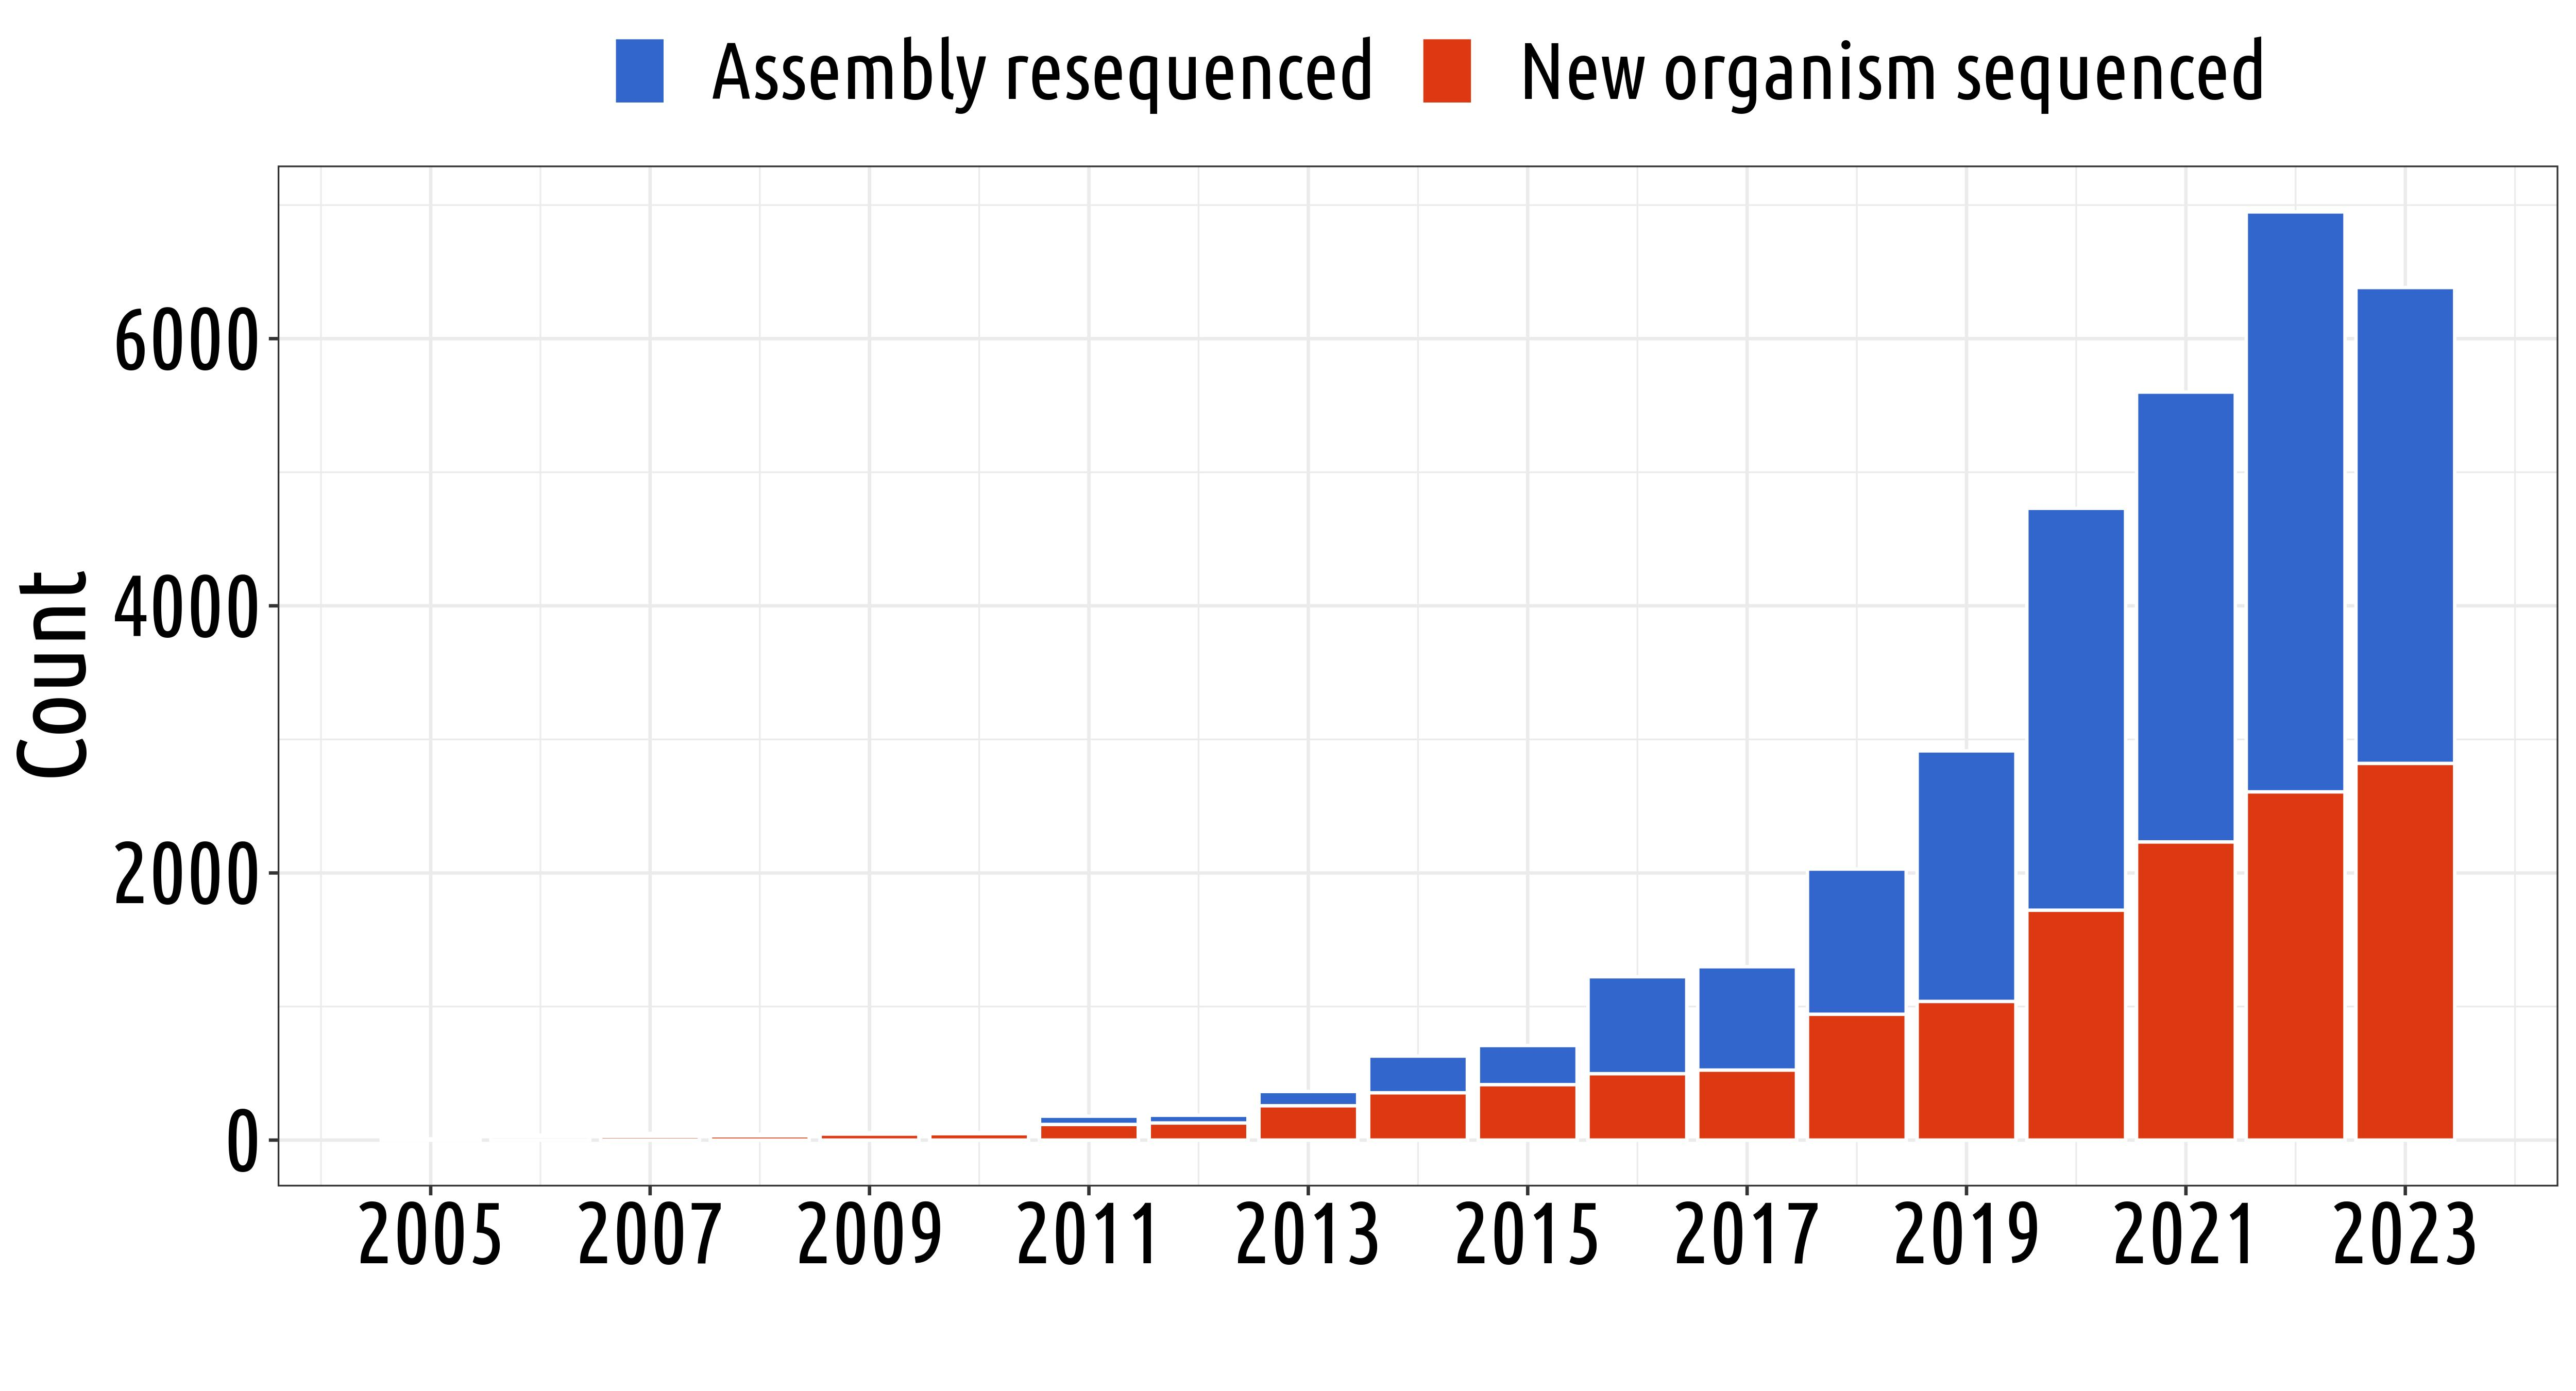
\includegraphics[width=\linewidth]{figures/nb_assembly_insdc.jpg}
    \caption[Yearly count of Eukaryota sequenced assemblies]{\textbf{Yearly count of Eukaryota sequenced assemblies.} This graph illustrates the annual deposition of Eukaryota genomes at the International Nucleotide Sequence Database Collaboration (INSDC), distinguishing between species deposited for the first time (red) and all assemblies (blue).\newline}
    \label{fig:nbassemblyinsdc}
\end{figure}

The latest advancements in third-generation sequencing techniques have culminated in long-read sequencing technologies, enabling the generation of reads of 1 to 20 kilobase~\citep{marx_method_2023, logsdon_long-read_2020}.

In addition, dedicated efforts have been directed towards sequencing the genomes of entire populations. This has facilitated the examination of genetic variations at a population level, contributing to our comprehension of the evolutionary forces that underlie these variations. The accumulation of extensive genetic data at this scale has opened novel avenues for investigating genetic diversity, population structure, adaptation, and mechanisms of evolution.

This growing number of genomes and transcriptomes sequenced poses new limitations related to the tremendous amount of data generated, that needs to be stored and archived. Also, new sequencing techniques use algorithms that require more and more resources (GPU, CPU, RAM...). Little by little the sequencing problem becomes now a bioinformatic problem.

\section{Evolution of Bioinformatics}

The term "bioinformatics" was originally introduced by Paulien Hogeweg and Ben Hesper in 1970 to denote the investigation of informational processes within biotic systems~\citep{hesper_bioinformatica_1970, hogeweg_roots_2011}. This designation emerged during a period when the volume of data and methodologies available necessitated the computational processing and analysis of substantial datasets that would have been impractical to handle manually. Bioinformatics has increasingly become an essential element in the field of biology. It involves employing computational and statistical methods to analyze, interpret, and manage biological data, particularly genetic and molecular information.

In recent years, significant progress has been made in bioinformatics, driven by enhanced computing power, the development of novel technologies, the improvement of analysis tools and algorithms. These advancements have expedited analyses, increased efficiency, and facilitated the management of ever-growing, intricate datasets. In this context, several algorithms and computer programs have been developed to study evolution.


\subsection{Sequences alignment}

The preceding section has discussed the burst of sequencing methods, followed by the inundation of genetic data in recent years. However, even in the 1970s, scientists had access to data pertaining not to \acrshort{DNA} sequences but rather to amino acid sequences of proteins. Notably, at the age of 37, Sanger achieved the sequencing of amino acid chains in bovine insulin, initially unraveling the initial 30 amino acids in chain B~\citep{sanger_amino-acid_1951, sanger_amino-acid_1951-1}, followed by 21 amino acids in chain A~\citep{sanger_amino-acid_1953, sanger_amino-acid_1953-1}. After investigation of insulin sequences across multiple species, the next challenge for Sanger was to align these sequences to establish correspondences between positions as they have undergone evolutionary changes. The premise underlying the comparative analysis of sequences from diverse species rested on the notion that conserved regions, retained throughout evolutionary processes, might indicate pivotal elements within the molecule, such as the `active center'. Notably, in his alignment Sanger observed that differences were confined to a discrete segment of the molecule~\citep{sanger_species_1949, brown_structure_1955, harris_species_1956}.

A multitude of methodologies have been devised to facilitate sequence alignments starting with pairwise alignment. The process of pairwise alignment involves aligning two sequences with each other. Among the noteworthy algorithms, the Needleman–Wunsch algorithm, introduced in 1970, stands out as one of the most renowned methods~\citep{needleman_general_1970}. This algorithm operates by constructing a matrix in which individual cells represent the optimal alignment score for specific subsequences. Through an iterative process, the algorithm populates the matrix, factoring in penalties for gaps and scores for similarity. The final alignment is determined by tracing back along the highest-scoring path within the matrix. It is particularly valuable for aligning closely related sequences of comparable lengths. Derivations of this alignment method have been made, notably with the introduction of the Smith–Waterman algorithm for local alignment~\citep{smith_identification_1981}. Local alignment focuses on identifying shorter, highly similar regions within sequences, accommodating gaps and mismatches outside these regions.

The next challenge was to align multiple sequences together, known as Multiple Sequence Alignment (MSA). These methods relies on a guide phylogenetic tree, which is a diagram illustrating the evolutionary descent of various species, organisms, or genes from a common ancestor, to guide the alignment process. This tree is computed using methods such as Neighbor Joining (NJ) based on a genetic distance matrix of the sequences~\citep{saitou_neighbor-joining_1987}. Following this tree sequences are successively incorporated to the MSA by pairwise alignment between sequences, a sequence and a consensus sequence or two consensus sequences.

After the creation of sequence databases, such as ACNUC~\citep{gouy_acnuc--portable_1985} or Genbank~\citep{burks_genbank_1991}, the need arose to compare a single sequence to a multitude of sequences. It became clear that comparing each pair would be a resource waste. To overcome this difficulty in 1985, the FASTA algorithm was developed, providing rapid search capabilities within protein databases~\citep{lipman_rapid_1985}. Subsequently, in 1990, it was succeeded by BLAST~\citep{altschul_basic_1990}. BLAST's core principle involves identifying short regions of high similarity (local alignments) between the query sequence and sequences within the database. BLAST's algorithm disassemble the query sequence into smaller fragments (k-mers), probing for these fragments within the database, and subsequently extending the matches into more extensive alignments. This methodology empowers BLAST to swiftly recognize regions of similarity without necessitating an exhaustive global alignment spanning the entire sequences' length. This focus on localized alignment makes BLAST an ideal choice for comparing sequences of varying lengths and identifying conserved regions, functional domains, and other biologically significant features. While BLAST predominantly hinges on local alignment principles, it's crucial to acknowledge the existence of alternative sequence alignment tools and algorithms that prioritize global alignment or adopt distinct alignment strategies tailored to specific bioinformatics objectives.

Around 2008, the emergence of transcriptomic sequencing data and their analyses required the alignment of billions of 100 \acrshort{bp} \acrshort{mRNA} reads to a reference genome~\citep{mortazavi_mapping_2008}. To do so, programs such as BOWTIE~\citep{langmead_ultrafast_2009}, TopHat2~\citep{kim_tophat2_2013} and HISAT~\citep{kim_graph-based_2019} have been developed. Unlike other alignment methods, these programs rely on a combination of k-mer indexing and graph-based alignment techniques. It creates a graph-like representation of the reference genome, facilitating alignment by accommodating various genomic variations, including single nucleotide polymorphisms (\acrshort{SNP}s), insertions, deletions, and splicing events. This approach ensures highly accurate and efficient alignment, particularly for RNA-seq data, where splicing events render local alignment less suitable. The incorporation of k-mer indexing enhances the speed and precision of the alignment process rendering possible gene expression estimation and alternative splicing analyses~\citep{kim_graph-based_2019}.


\subsection{Collaborative science in the era of big data}

Research and collaborative science play a crucial role in the field of genome biology, especially concerning the utilization of massive datasets. The surge in data acquisition, driven by cost efficiencies and technological advancements, has not only spurred cooperative efforts and the exchange of data but has also facilitated large-scale studies. This enables the effective utilization of genetic insights across diverse domains of evolutionary biology.

In response to the arising amount of DNA/RNA sequencing data, instances have created database as an answer to store and use these genetic data. In Europe the European Molecular Biology Laboratory (\acrshort{EMBL}) created the \acrshort{EMBL} Data Library as a repository for genetic information in 1980~\citep{hamm_embl_1986}. By 1982, this database encompassed 568 sequence entries~\citep{kneale_embl_1984}. Subsequently, in 1990 the \acrshort{EMBL} Data Library was relocated at the European Bioinformatics Institute (\acrshort{EBI}) and renamed \acrshort{EMBL} Nucleotide Sequence Database~\citep{rodriguez-tome_european_1996}. In response to the advent of Next Generation Sequencing (NGS) data, the European Nucleotide Archive (\acrshort{ENA}) emerged in 2008 through the fusion of the \acrshort{EMBL} Nucleotide Sequence Database and the former Sequence Read Archive (SRA)~\citep{leinonen_european_2011}.

\begin{figure}[h]
    \centering
    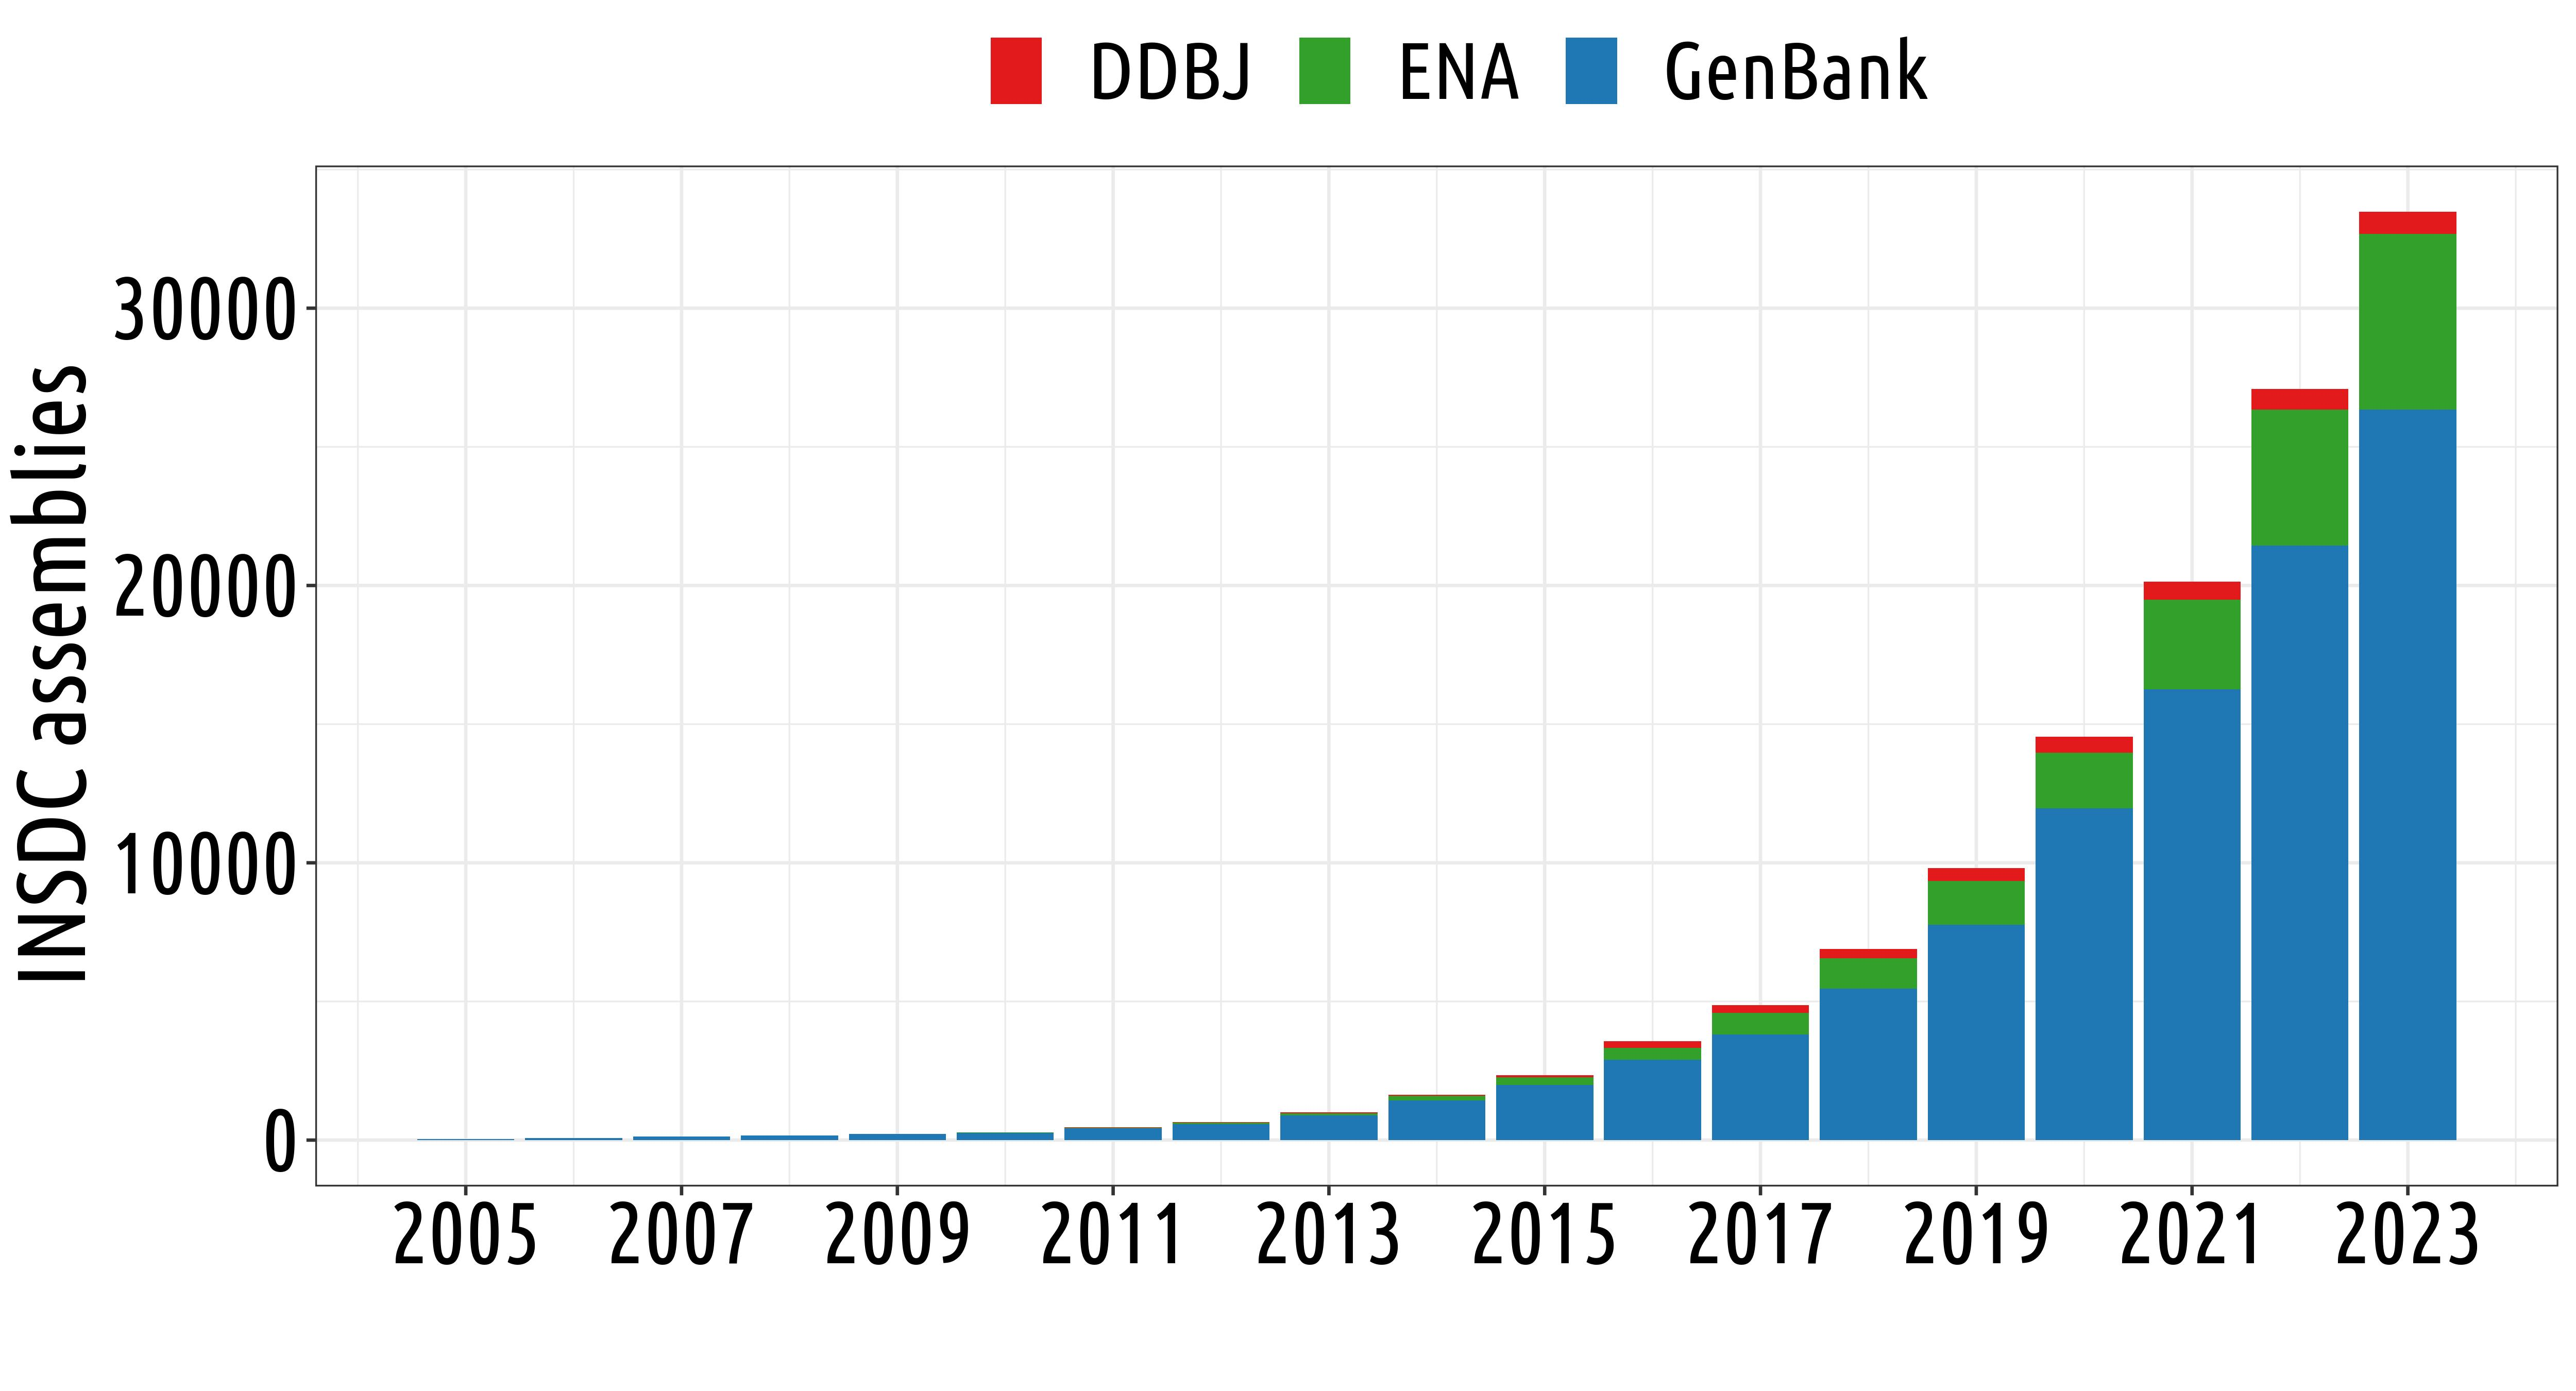
\includegraphics[width=.7\linewidth]{figures/nb_assembly_per_db_insdc.jpg}
    \caption[Annual INSDC contributions by structures]{\textbf{Annual INSDC contributions by structures.} Annual deposition of Eukaryota assemblies in distinct partner members of the International Nucleotide Sequence Database Collaboration (INSDC): National Center for Biotechnology Information (\acrshort{NCBI}) (depicted in blue), DNA Data Bank of Japan (DDBJ) (depicted in red), and European Nucleotide Archive (\acrshort{ENA}) (depicted in green).\newline}
    \label{fig:nbassemblyperdbinsdc}
\end{figure}

In the United States, the GenBank sequence database was established in 1982~\citep{sayers_genbank_2022}. During 1989 to 1992, the GenBank initiative transitioned to the National Center for Biotechnology Information (\acrshort{NCBI};~\citet{ncbi_resource_coordinators_database_2018}). Similarly, in 1987, the DNA Data Bank of Japan (DDBJ) pioneered the sole nucleotide sequence data repository in Asia~\citep{tateno_dna_1997}.  From their inception, these three databases have maintained a collaborative methods, giving rise to the International Nucleotide Sequence Database Collaboration (INSDC) in 2005~\citep{karsch-mizrachi_international_2012}. Daily, the DDBJ/EMBL/GenBank consortium engages in the exchange of data submissions and mutual data sharing (\citet{brunak_nucleotide_2002}; \hyperref[fig:nbassemblyperdbinsdc]{Fig. 3.2}). Currently, these databases collectively house data from nearly 14,000 eukaryota genomes, with new submissions pouring in daily (\hyperref[fig:nbspeciesinsdc]{Fig. 3.3}). Beyond genome sequences, these databases host a wealth of information, including annotations, protein and coding sequences. Moreover, they serve as repositories for diverse non-sequence-related data such as species taxonomy information.

\begin{figure}[h]
    \centering
    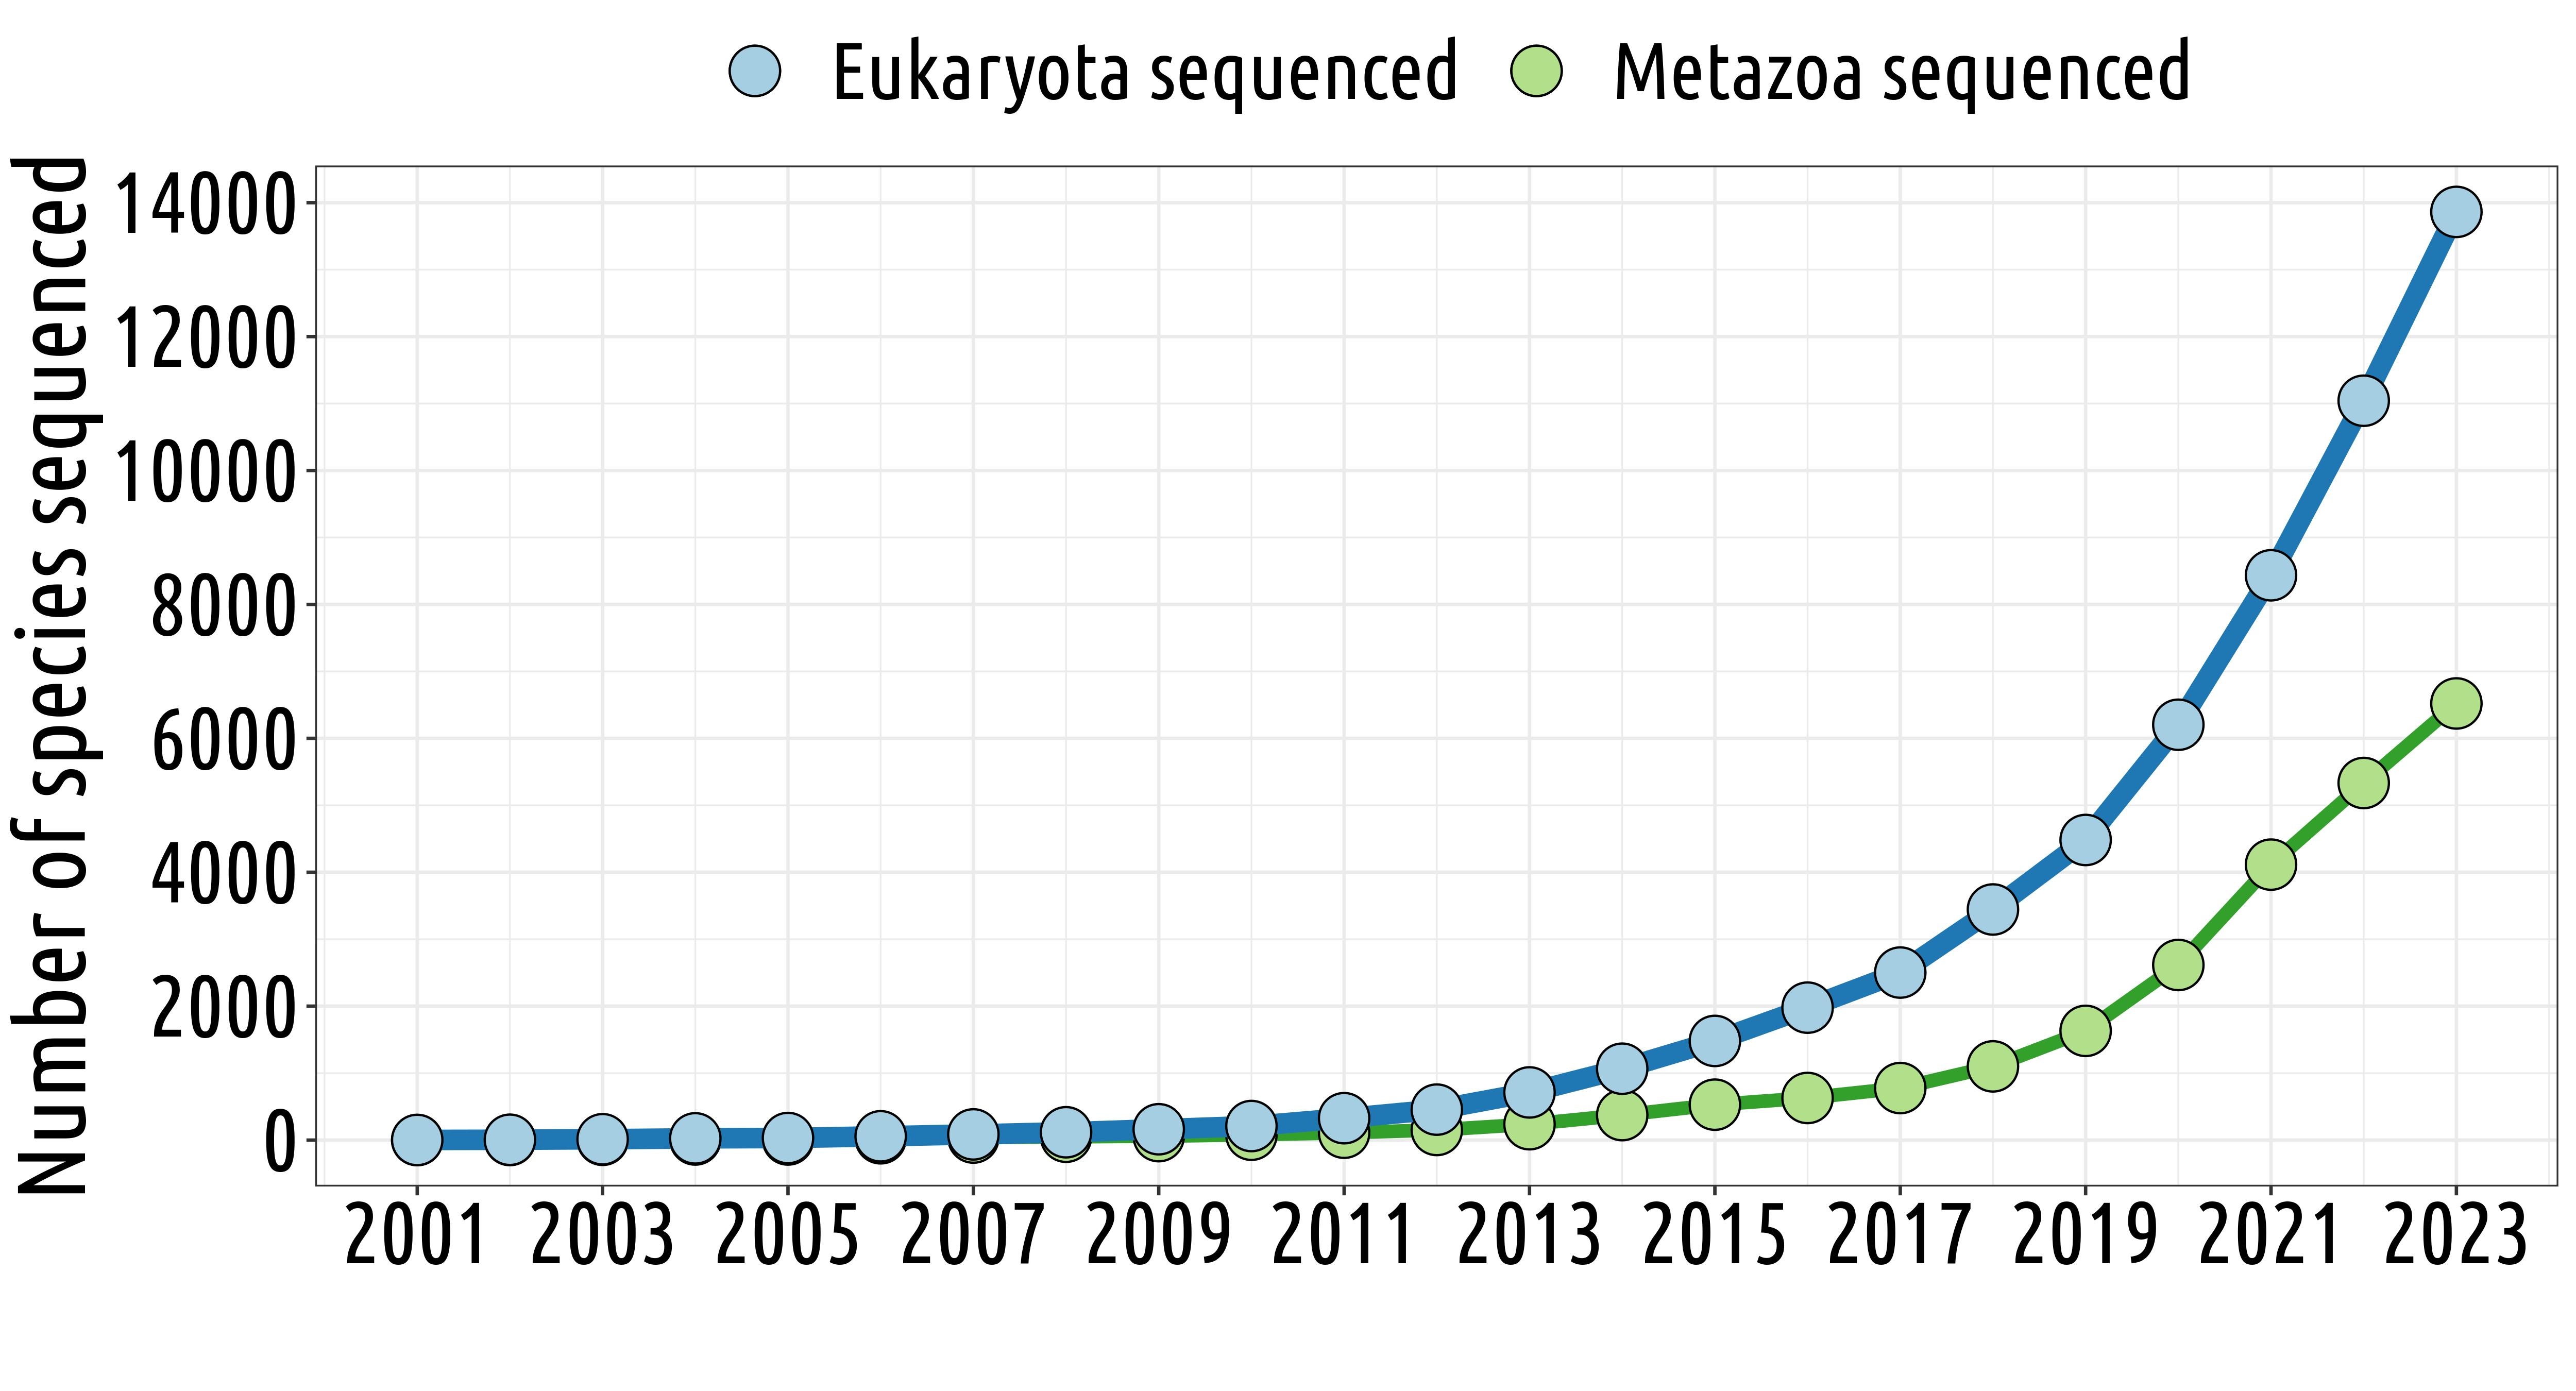
\includegraphics[width=.7\linewidth]{figures/nb_species_insdc.jpg}
    \caption[Number of species sequenced over time on INSDC]{\textbf{Number of species sequenced over time on INSDC.} This figure depicts the number of species' genome sequenced available at the International Nucleotide Sequence Database Collaboration over time. Eukaryota (blue); Metazoa (green).\newline}
    \label{fig:nbspeciesinsdc}
\end{figure}

Also, the \acrshort{BUSCO} annotation program, provides datasets of single-copy orthologous genes for diverse species clades and is derived from the database OrthoDB \citep{kuznetsov_orthodb_2023, manni_busco_2021}. OrthoDB database is a comprehensive resource containing single-copy orthologous genes for a wide range of clades. OrthoDB delineates orthologs at key points along the species phylogeny, corresponding to the last common ancestor of the species being studied.

In addition to DNA sequencing data, an abundance of other data sources has given rise to a multitude of specialized databases. For instance, the Human Ageing Genomic Resources integrated the AnAge database in 2013, providing data on life history traits in animals, encompassing aspects like maximum longevity, body mass, gestation, and sexual maturity~\citep{tacutu_human_2013, tacutu_human_2018}. The Encyclopedia of Life (EOL), hosted by the National Museum of Natural History Smithsonian, became operational in 2014, consolidating information on parameters such as body length, body mass, longevity, and species distribution~\citep{wilson_encyclopedia_2003, parr_encyclopedia_2014}. Similarly, the Animal Diversity Web, an online compendium of animal natural history, classification, and conservation biology, has been collaboratively assembled and is maintained by the Museum of Zoology at the University of Michigan~\citep{myers_animal_2023}.

The proliferation of databases continues unabated (\hyperref[fig:narbiodb]{Fig. 3.4}), and a database of molecular biology database is kept updated by Nucleic Acids Research (NAR). It lists the databases that have been described in the annual NAR database issues~\citep{rigden_2018_2018, rigden_2023_2023}. The latest Issue contains 178 papers ranging across biology and related fields, and the NAR online Molecular Biology Database Collection presently encompasses an impressive tally of 1,764 databases.

\begin{figure}[h]
    \centering
    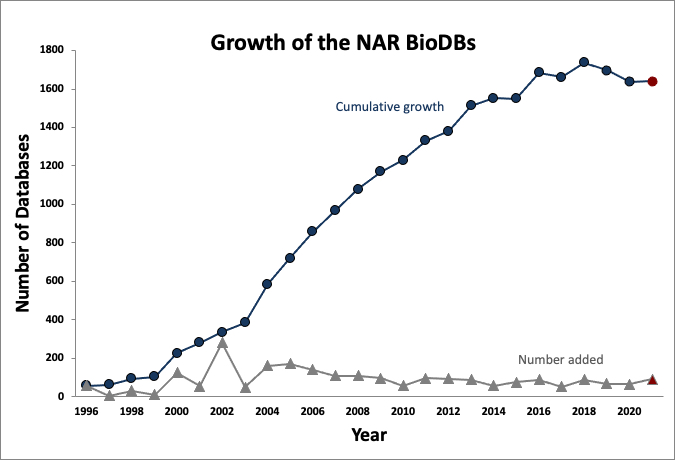
\includegraphics[width=.7\linewidth]{figures/nar_biodb.jpg}
    \caption[Expansion of Nucleic Acids Research Database]{\textbf{Expansion of Nucleic Acids Research Database.} Cumulative growth of the NAR BioDBs described in the annual NAR database issues. Obsoletes and discontinued databases are removed each year. \\
    \scriptsize{Reproduced with permission from Sandra Porter, president of Digital World Biology.}}
    \label{fig:narbiodb}
\end{figure}
% \url{https://digitalworldbiology.com/blog/bio-datatabases-2021-sars-cov-2-antibody-structures}
These databases collectively encompass an array of data domains, spanning gene composition, expression patterns, protein sequences, genomic information, cancer studies, plant and metazoan biology, gene orthologs, life history traits, and taxonomy, thereby constituting invaluable resources for researchers across disciplines. However, they inexorably generate such a quantity of data that we no longer know what to do with it. With data resources that are scattered, holed and sometimes annotated inconsistently. They are therefore difficult to reconcile in order to do coherent, reproducible and systemic analyses. A world where everyone has to redo their analyses from the beginning due to the publication of new datasets, new methods, new algorithms, without an integrative structure.